\chapter{Estado del Arte}
\label{sec:EstadoDelArte}
La estimación de calidad de imágenes y objetos 3D, al ser un componente sumamente 
ligado al avance tecnológico y necesidades de manejo de información digital, ha 
tomado mayor interés en el comienzo del siglo actual.
Puede observarse en la Figura \ref{fig:ScopusMLinMedicalAndPC} que existe 
una tendencia creciente en el número de publicaciones en relación a la aplicación 
de inteligencia artificial en las nubes de puntos y en imágenes médicas, llegando
ambas a sobrepasar 6000 documentos a partir de 2020.  Vemos que ambos incluso siguen 
lado al lado en número de publicaciones cuando especificamos que sean documentos 
relacionados con la estimación de calidad, sobrepasando los 250 documentos. 
Por otro lado, y afirmando lo mencionado sobre el bajo número de publicaciones 
en el ámbito biomédico para la estimación de calidad en 3D, vemos que, aunque hay
también una tendencia positiva, en 2022 tenemos solo 62 publicaciones. Esto 
se interpreta como indicador de lo novedoso y pionero de este proyecto.
\footnotetext[1]{
  Las búsquedas se pueden consultar en el Apéndice \ref{subs:Scopus}
}
\begin{figure}[H]
  \centering
  \begin{subfigure}{0.49\textwidth}
    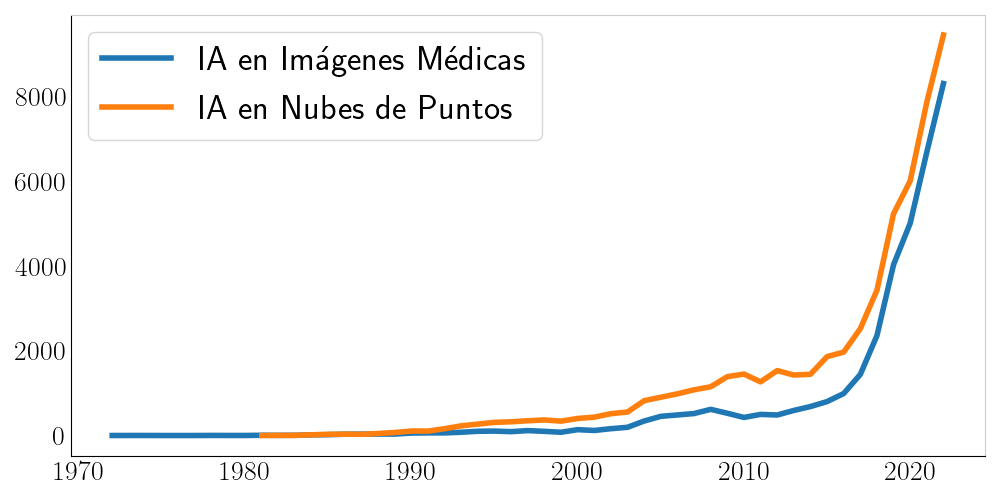
\includegraphics[width=\textwidth]{imagenes/chapter3/ScopusMLinMedicineAndPC.png}
  \end{subfigure}
  \begin{subfigure}{0.5\textwidth}
    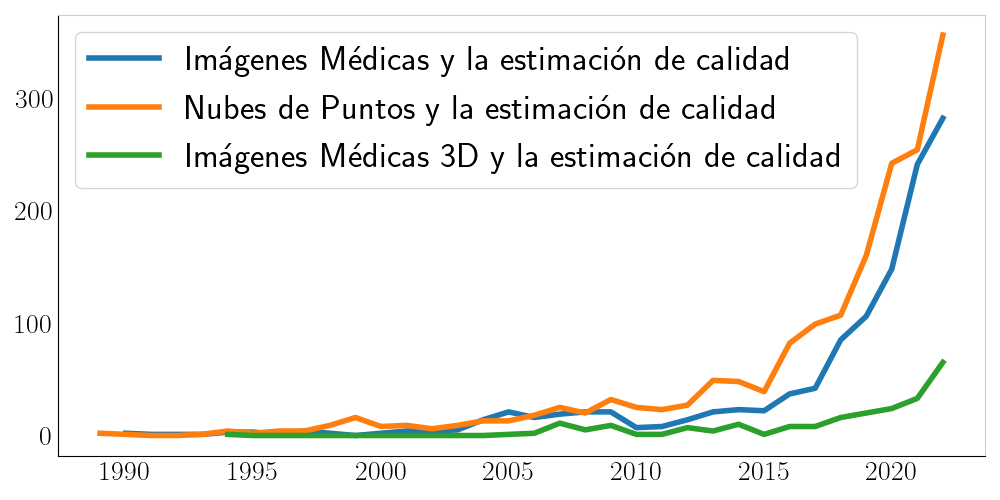
\includegraphics[width=\textwidth]{imagenes/chapter3/ScopusQualityAssessment.png}
  \end{subfigure}
  \caption[Crecimiento de interés en el campo según \emph{Scopus}]{Crecimiento de interés en el campo según \emph{Scopus}\footnotemark[1].
  A la izquierda podemos ver un incremento de publicaciones desde 
  1970 sobre la IA aplicada a nubes de punto, en naranja, 
  y aplicada de forma general a imágenes médicas, en azul. A la derecha 
  podemos ver de forma similar el crecimiento de métodos aplicados
  a la estimación de calidad a nubes de puntos, naranja, a imágenes médicas, azul, y 
  a imágenes médicas 3D, verde.
  }
  \label{fig:ScopusMLinMedicalAndPC}
\end{figure}
A continuación se presenta el estado del arte. Comentaremos, brevemente, el 
estado actual de los métodos IQA tradicionales. A continuación,
el estado de métodos en imágenes médicas 2D. Y por último, nos centraremos 
en el estado actual de métodos sin referencia para nubes de puntos, el campo 
sobre el cual trabajaremos.

\section{Estado del arte de FR-IQA}
Como ha sido mencionado anteriormente, los métodos convencionales de cuantificación del error en la evaluación de la fidelidad 
de imágenes, como el error cuadrático medio, la relación señal-ruido (SNR, por sus siglas en inglés) y el pico de señal-ruido (PSNR, por su siglas en inglés), 
no consideran el contenido de una imagen ni las características del sistema visual 
humano (HVS, por sus siglas en inglés). Por lo tanto, estos métodos suelen tener 
una débil consistencia con la percepción humana, recordar Figuras\ref{fig:FailureMinkowskiMetric} y \ref{fig:MSEHyperSphere}. 
Para abordar esta limitación, se han propuesto métricas inspiradas en el HVS y 
conscientes del contenido de la imagen, que combinan las características del HVS con algoritmos matemáticos. 
Por ejemplo, Visual SNR\cite{VSNR} que cuantifica la fidelidad visual de las imágenes 
distorsionadas, mientras que PSNR-HVS\cite{PSNR-HVS} combina el PSNR con las 
características del HVS al considerar la función de sensibilidad al contraste. 

Wang y Bovik afirmaron que los ojos humanos obtienen información de imagen a través de tres canales: brillo, contraste y estructura\cite{SSIM}, 
y desarrollaron un índice universal de calidad de imagen (UQI)\cite{UQI} y una similitud estructural (SSIM, por sus siglas en inglés)\cite{SSIM}.
Desde entonces, se han propuesto diversas variantes basadas en SSIM, como MS-SSIM\cite{MS-SSIM}.
Surgieron también métodos que, basados en las respuestas del HVS, introducen la 
saliencia visual\footnote{
  Cualidad estética de la forma de un objeto o una configuración que destaca.
}en la evaluación de la calidad de imagen (VSI)\cite{VSI}, 
ya que se ha observado que la saliencia de la imagen desempeña un papel importante.

En los últimos años, se han aplicado métodos de aprendizaje automático. 
Algunos ejemplos de estos métodos son MLIQM\cite{MLIQM}, que clasifica las imágenes distorsionadas en 
cinco escalas utilizando máquinas de soporte vectorial (SVM, por sus siglas en inglés), y MMF\cite{MMF} que utiliza 
una fusión multimétodo motivada por la observación de que ningún método único puede ofrecer 
el mejor rendimiento en todos los tipos de distorsión.
Además, se ha llegado a utilizar incluso CNN's para resolver el problema, ya que son capaces de aprender características 
y regresión a partir de los datos brutos de las imágenes. Un ejemplo de esto es 
WaDIQaM-FR\cite{DIQaM}, que es una medida de calidad de imagen profunda ponderada y 
basada en datos sin depender de características predefinidas o conocimiento previo.

\begin{table}[htp]
  \tiny
  \hspace{-1.8cm}
  \begin{tabular}{|c|c|c|c|c|c|c|c|c|c|c|c|c|c|}
    \hline
    \rowcolor[HTML]{FFC702}
    & &  \multicolumn{3}{c|}{LIVE}& \multicolumn{3}{c|}{\textbf{CSIQ}} & \multicolumn{3}{c|}{\textbf{TID2008}} & \multicolumn{3}{c|}{\textbf{TID2013}} \\ 
    \cline{3-14}\noalign{\vskip.1pt}
    \rowcolor[HTML]{FFC702}
    \multirow{-2}{*}{\textbf{Type}} & \multirow{-2}{*}{\textbf{Metric}} & SRCC & PLCC & RMSE & SRCC & PLCC & RMSE & SRCC & PLCC & RMSE & SRCC & PLCC & RMSE \\
    \hline
    \multirow{10}{*}{FR}
                   & VSNR\cite{VSNR} & 0.927 & 0.923 & 10.506 & 0.811 & 0.800 & 0.158 & 0.705 & 0.682 & 0.982 & 0.681 & 0.740 & 0.839 \\
                   & PSNRHVS\cite{PSNR-HVS} & 0.919 & 0.903 & 12.540 & 0.830 & 0.804 & 0.156 & 0.594 & 0.608 & 1.065 & 0.654 & 0.430 & 0.704 \\
                   & UQI\cite{UQI} & 0.894 & 0.899 & 11.982 & 0.810 & 0.831 & 0.146 & 0.585 & 0.664 & 1.003 & - & - & -\\
                   & SSIM\cite{SSIM} & 0.948 & 0.845 & 8.946 & 0.876 & 0.861 & 0.133 & 0.775 & 0.773 & 0.851 & 0.742 & 0.790 & 0.761\\ 
                   & MS-SSIM\cite{MS-SSIM} & 0.951 & 0.949 & 8.169 & 0.913 & 0.899 & 0.115 & 0.854 & 0.845 & 0.717 & 0.786 & 0.833 & 0.686\\
                   & VSI\cite{VSI} & 0.952 & 0.948 & 8.682 & 0.942 & 0.928 & 0.098 & 0.898 & 0.876 & 0.647 & 0.897 & 0.900 & 0.540\\
                   & DSS\cite{DSS} & 0.962 & 0.931 & 9.961 & 0.961 & 0.957 & 0.076 & 0.873 & 0.877 & 0.644 & 0.792 & 0.848 & 0.658\\
                   & CD-MMF\cite{MMF} & \textbf{0.981} & \textbf{0.980} & \textbf{5.413} & \textbf{0.967} & \textbf{0.9614} & \textbf{0.067} & \textbf{0.942} & \textbf{0.9414} & \textbf{0.429} & - & - & -\\
                   & WaDIQaM-FR\cite{DIQaM} & \textbf{0.970} & \textbf{0.980} & - & - & - & - & - & - & - & \textbf{0.940} & \textbf{0.946} & -\\
                  \hline 
  \end{tabular}
  \caption[Tablas estado del arte FR-IQA]{Tabla extraída de \cite{SurveyOf2D3DMetrics}, 
    donde vemos el progreso de las métricas FR conforme avanza los conocimientos
  del HVS, ML y DL.}
    \label{tab:SOTAFRIQA}
\end{table}

\section{Estado del arte de NR-IQA}
Al principio, surgieron métricas para la estimación de la calidad de las imágenes 
que hubiesen sufrido algún tipo de distorsión específica, 
como imágenes borrosas\cite{GradientBasedBlurAssessment}, 
imágenes comprimidas en JPEG\cite{JPEGBasedOnLuminance}, 
imágenes con artefactos de bloque\cite{DeblockedImages} y imágenes con cambios de contraste\cite{ContrastDistorted}.
Luego, se buscaron maneras de estimar la calidad de imágenes de forma más genérica, 
sin depender del tipo de distorsión. Para ello, se han propuesto varias métricas 
basadas en estadísticas de escenas naturales (NSS, por sus siglas en inglés). 
Un ejemplo conocido es el evaluador sin referencia BRISQUE\cite{BRISQUE}, que extrae 
características NSS de un modelo estadístico de coeficientes de luminancia 
normalizados localmente en el dominio espacial y demuestra que estas características 
se correlación bien con las evaluaciones humanas.
También se han presentado métricas basadas en aprendizaje automático, 
como el índice basado en patrones locales de gradiente LGP\cite{LGP} que extrae 
características estadísticas locales de la magnitud y fase del gradiente de la imagen y utiliza una 
SVM para mapear la calidad subjetiva de la imagen a 
características estadísticas locales que transmiten información estructural importante.
Recientemente, las redes neuronales convolucionales se han introducido con 
éxito en el campo de la evaluación de la fidelidad de imágenes sin referencia. 
Se propuso un trabajo pionero llamado IQA-CNN\cite{IQA-CNN}, 
y posteriormente se han realizado muchos esfuerzos para mejorar su rendimiento 
mediante el diseño de estructuras convolucionales más profundas. En concreto,
DIQaM-NR\cite{DIQaM}, que mejora frente redes menos profundas.

\begin{table}[htp]
  \tiny
    \centering
    \begin{tabular}{|c|c|c|c|c|}
    \hline 
    \rowcolor[HTML]{FFC702}
    & & \multicolumn{3}{c|}{\textbf{LIVE}}\\
   \cline{3-5}\noalign{\vskip.1pt}
    \rowcolor[HTML]{FFC702}
      \multirow{-2}{*}{\textbf{Type}} & \multirow{-2}{*}{\textbf{Metric}} & SRCC & PLCC & RMSE \\
    \hline
    \multirow{5}{*}{NR} & 
                           BRISQUE \cite{BRISQUE} & 0.940 & 0.942 & - \\
                          & LGP \cite{LGP} & 0.957 & 0.954 & 7.901 \\
                          & IQA-CNN \cite{IQA-CNN} & 0.956 & 0.953 & - \\
                          & DIQaM-NR \cite{DIQaM} & \textbf{0.960} & \textbf{0.972} & - \\
                          & Hallucinated-IQA \cite{Hallucinated-IQA} & \textbf{0.982} & \textbf{0.982} & - \\
                          \hline
  \end{tabular}
  \caption[Tablas estado del arte NR-IQA]{Tabla extraída de \cite{SurveyOf2D3DMetrics}, 
    donde vemos el progreso de las métricas NR al utilizar métodos cada vez más complejos.}
  \label{tab:SOTANRIQA}
\end{table}

\section{Estado del arte de IQA en imágenes médicas}

En el caso de la evaluación de calidad FR y RR, se requiere disponer 
de una imagen de referencia sin distorsión o una parte de una imagen con la cual 
se pueda comparar la imagen evaluada. Sin embargo, en el caso de las imágenes médicas, 
no existe una imagen sin distorsión\cite{DicomDistortionsExample}. 
Por lo tanto, el desarrollo de métodos de evaluación de calidad de imágenes 
sin referencia es de particular importancia en este campo\cite{LGP, BRISQUE, IQA-CNN, DIQaM, Hallucinated-IQA}.
Como fue mencionado, la salida de estos algoritmos pueden ser utilizados 
para filtrar imágenes de baja calidad en un gran conjunto de imágenes médicas o 
para ayudar a mejorar su calidad, siendo esta crucial para el diagnóstico\cite{DicomDistortionsExample}.
Predominantemente, el conocimiento del ámbito de la imagen es crítico para estimar 
su calidad. Es por ello que la mayoría de los métodos actuales son para un tipo específico 
de examen médico o distorsión.

Por ejemplo, basándose en el sistema visual humano (HVS), 
Bhateja et al.\cite{MultiModalMRIFusionMethod} utilizaron métricas de fusión
de imágenes de resonancia magnética (MRI) de dos etapas para IQA.
Con el objetivo de desarrollar métodos automáticos de aprendizaje profundo,
Xu et al.\cite{SemiSupervisedMRIFetalBrain} introdujeron una técnica semi-supervisada dedicada a la evaluación de 
calidad de imágenes de MRI cerebral fetal utilizando un método de 
profesor promedio\footnote{
Método de aprendizaje semi-supervisado que utiliza dos modelos, 
uno considerado estudiante y otro profesor, que trabajan conjuntamente para aprender
a resolver la tarea.
} y la consistencia de las regiones de interés. 
Además, Liu et al.\cite{IQAForPediatricMRIWithNoisySegmentation}utilizaron el aprendizaje semi-supervisado para resolver 
el problema de crear anotaciones ruidosas en la tarea de segmentación de imágenes. 
Esta técnica de evaluación de calidad de tres etapas utiliza un modelo residual 
jerárquico y proporciona una evaluación a nivel de corte, volumen y sujeto. 

Otro método de estimación utiliza una red generativa adversaria no emparejada 
y un clasificador entrenado débilmente supervisado para evaluar imágenes MRI\cite{MIGAN}.
Para abordar el problema de desperdiciar información espacial 3D potencialmente importante, 
se creó el enfoque HyS-net\cite{Hys-net}, basado en una hiper-red y que es capaz de 
auto adaptación. Así como fue expuesto anteriormente, no es posible 
simplemente implementar métodos IQA, es por ello que Chow y Rajagopal \cite{MedicalBRISQUE} 
propusieron un enfoque más reciente que adapta el evaluador de calidad de imagen más famoso BRISQUE\cite{BRISQUE}.

Hay que tener en cuenta que la explicabilidad es un aspecto crucial 
para evaluar la fiabilidad de los sistemas de diagnóstico automático, 
especialmente en aplicaciones de aprendizaje profundo tipo caja negra. 
Dado que un clasificador profundo nos proporciona solo el valor inferido 
para un escaneo médico dado, es imperativo descubrir las señales que pueden 
ayudar a asegurar que la decisión se haya tomado en función de conjuntos de 
características relacionales.

\section{Estado del arte de FR-PCQA}
Las métricas más populares para la estimación objetiva de la calidad de modelos 
3D basada en puntos son \emph{point-to-point} (Po2Po)\cite{PointToPoint} y
\emph{point-to-plane} (Po2Pl)\cite{PointToPlane}. 
En la primera, para cada punto del objeto distorsionado se obtiene su vecino más cercano en la versión de referencia y 
se calcula alguna métrica de distancia como las discutidas anteriormente (MSE, Minkowski, Hausdorff...). 
La principal desventaja de estos modelos es que no consideran los objetos como 
superficies.

Para solventar este problema se formuló el segundo método por Tian et al. 
que modela la superficie en cada punto como un plano. 
Ese plano es perpendicular a la normal en cada punto, que se calcula en base a la información de su vencindario. 
Se propuso también otra métrica como \emph{Plane-to-Plane} (Pl2Pl)\cite{PlaneToPlane}, 
que mide la similitud entre superficies asociadas a las nubes de puntos. Dentro 
de este mismo ámbito surge también \emph{Point-to-Surface}\cite{PlaneToSurface}, 
que mide la distancia de cada punto de la versión distorsionado respecto a su 
superficie correspondiente en la nube de referencia. Luego para poder tener en
cuenta los colores, surgieron métricas como Po2Po PSNR donde la diferencia 
ya no es respecto a la posición del punto sino que al color.
%en el espacio $YC_bC_r$.

De la información del vecindario de los puntos, gran cantidad de información geométrica 
puede ser extraída para investigar en profundidad la similitud entre las nubes 
de puntos. Surgieron métodos basados en la extracción de características donde la 
mayoría considera tanto información geométrica como los atributos lumínicos.
Un ejemplo sería PointSSIM\cite{PointSSIM}, una métrica que busca la similitud estructural entre nubes de puntos basándose en
las estadísticas locales de curvatura de los puntos, junto a la información 
extraída de los colores, como adaptación del método SSIM\cite{SSIM}.
Experimentando con combinaciones de 3 medidas geométricas y 5 comparaciones de color 
para encontrar el mejor vector características resultó en la métrica PCQM\cite{PCQM}.
% Similar, utilizando el análisis de componentes principales (PCA) en un vecindario 
% de puntos para extraer los valores y vectores singulares por cada punto permitió 
% obtener buenos descriptores de información geométrica\cite{PointPCA}.

% También se estudió las componentes lumínicas de las nubes de puntos en \cite{ColorBasedObjectiveMetricPC, BitDance}. 
% Consistía en generar un histograma y correlograma de la componente lumínica. 
% Un correlograma nos permite caracterizar la relación entre pares de variables 
% numéricas en un conjunto de datos. 
Otros, velaron por estudio la energía potencial en las nubes de puntos y 
las diferencias que emergen en presencia de distorsiones (MPED)\cite{MPED}.
Por otro lado, utilizando transformaciones de datos, se construyeron grafos que representan 
las nubes de puntos, tanto la de referencia como la distorsionada, 
para producir métricas de similitud como GraphSIM\cite{GraphSIM}.
De igual forma se adaptaron ideas de otros ámbitos, por ejemplo, utilizando 
proyecciones que trasladan el mundo tridimensional a un espacio 2D para utilizar 
los métodos más conocidos de estimación de calidad en imágenes.
Se realizó incluso un estudio sobre el impacto del número de proyecciones 2D de 
distintas perspectivas en el rendimiento de las métricas de calidad\cite{ImpactOf2DProyections, IT-PCQA}.

Conocer algunas de estas métricas del estado del arte de los métodos con referencia nos 
servirá a la hora de generar el conjunto de datos sintéticos para la evaluación 
del modelo sobre imágenes médicas 3D, ver Sección \ref{sec:DatosSinteticos}. 

\section{Estado del arte de NR-PCQA}
Los métodos de evaluación de fidelidad de imágenes 3D NR tienen más perspectivas 
de aplicación práctica que los métodos FR, ya que no utilizan ninguna información 
adicional del objeto de referencia.
El enfoque común para este problema es el uso de métricas basadas en 
aprendizaje, donde se crea un modelo de predicción basado en propiedades de la 
nube de puntos que se creen relacionadas con la calidad de percepción.

Al igual que en las primeras aproximaciones de los métodos NR-IQA, existen 
algoritmos de estimación específicos, como el propuesto por Liu et al\cite{bitstreamPCQ},
método centrado en predecir la calidad de nubes de puntos 
codificadas mediante V-PCC, algoritmo de compresión, utilizando un modelo NR 
a nivel de \emph{bitstream}. A continuación, los métodos siguen el camino explorado 
por los métodos FR-PCQA extrayendo características de las nubes de puntos para 
entrenar modelos.  Chetouni et al.\cite{NR-CNN-3D-PC} utilizó distancias geométricas, curvaturas medios 
y niveles de color, en escala gris. Zhang et al.\cite{NR3DQA} siguiendo la misma 
línea extrajo características de los vectores y valores singulares de cada punto,
además de utilizar características lumínicas.

El siguiente paso, al igual que en FR, se empezó a investigar la posibilidad 
de utilizar proyecciones 2D. En PQA-Net\cite{PQA-Net} se realiza un mapeado 
utilizando una estrategia de proyección multi-vista para extraer un vector de 
características de 384 dimensiones, que alimenta a dos módulos de aprendizaje 
que calculan conjuntamente la calidad de la nube de puntos degradada. 
En IT-PCQA\cite{IT-PCQA} deciden utilizar métodos IQA aplicadas a las multi-proyecciones.
Extendiendo los trabajos anteriores, tenemos VQA-PC\cite{VQA-PC} que trata las 
multi-proyecciones como vídeo, pudiendo así utilizar información espacial, 
imágenes en posiciones específicas, y información de consistencia temporal 
de la nube de puntos rotando. 

Los últimos pasos deciden utilizar información de la nube de puntos, para 
entender remediar cierta pérdida de información que puede ocurrir al proyectar-la. 
En ResSCNN\cite{ResSCNN} modifican el esqueleto de PointNet\cite{PointNet} para 
utilizar convoluciones dispersas, extraer características de forma jerárquica y 
predecir la calidad de la nube. También, con intención de ayudar al desarrollo 
de métodos NR-PCQA de aprendizaje profundo, construyeron el mayor conjunto de datos
de nubes de puntos sintético, en el momento de escritura, con su estimación de calidad. 
Otro método que trabaja directamente sobre la nube de puntos es SGR\cite{SGR}, 
que extraen regiones locales de la nube de puntos y analizan la calidad de los parches.
Recientemente, ha salido el modelo MM-PCQA\cite{MM-PCQA} que utilizan tanto información 
directa de la nube de puntos como información de las proyecciones. Incluso, hay 
métodos que han optado por utilizar un \emph{ensemble}\cite{EnsemblePCQA} de 
modelos pre-entrenado en 2D y obtuvieron muy buenos resultados. 

\begin{table}[H]
    \centering
    \small
    \begin{tabular}{|c|c|c|c|c|}
        \hline
        \rowcolor[HTML]{FFC702}& \multicolumn{2}{c|}{\textbf{STJU-PCQA}} & \multicolumn{2}{c|}{\textbf{WPC}} \\ \cline{2-5}\noalign{\vskip.2pt}
        \multirow{-2}{*}{\cellcolor[HTML]{FFC702}\textbf{MODELO}}  &\cellcolor[HTML]{FFC702} PLCC & \cellcolor[HTML]{FFC702}SRCC & \cellcolor[HTML]{FFC702}PLCC & \cellcolor[HTML]{FFC702}SRCC\\
        \hline
        MM-PCQA\cite{MM-PCQA} & 0.92 & 0.91 & 0.83 & 0.83\\
        \hline
        SGR\cite{SGR} & 0.89 & 0.84 & - & - \\
        \hline
        VQA-PC\cite{VQA-PC} & 0.8635 & 0.8509 & 0.7976 & 0.7968\\
        \hline
        ResSCNN\cite{ResSCNN} & 0.86 & 0.81 & 0.72 & 0.75\\
        \hline
        GPA-Net\cite{GPA-NET} & 0.806 & 0.78 & - & - \\
        \hline
        Zhang et al.\cite{NR3DQA}& 0.7382 & 0.7144 & 0.6514 & 0.6479\\
        \hline
        IT-PCQA \cite{IT-PCQA}& 0.58 & 0.63 & 0.55  & 0.54\\
        \hline
        % bitstreamPCQ\cite{bitstreamPCQ} & ? & ? & ? & ?\\
        % \hline
        % PQA-Net\cite{PQA-Net} & ? & ? & ? & ?\\
        % \hline 
        % Chetouni et al.\cite{NR-CNN-3D-PC}& ? & ? & ? & ? \\
        % \hline
    \end{tabular}
    \caption[Estado del arte de modelos NR-PCQA]{Resumen del estado del arte de modelos NR-PCQA en dos datasets muy conocidos: SJTU\cite{SJTU} y WPC\cite{WPC1,WPC2}.}
\end{table}

\Brian[{Sobre estimación de calidad en imágenes médicas 3D}]{Aunque en la Figura
\ref{fig:ScopusMLinMedicalAndPC} parece haber documentos para la estimación de 
calidad de imágenes médicas 3D, solamente encontré uno respecto a la calidad 
de segmentaciones. Los demás, imagino que son apenas documentos que contienen la palabra calidad o estimación. 
Así que no sé exactamente si dedicar una sección a decir que no he encontrado 
nada o qué decir aquí.}

